\section{Thesis outline}

\begin{wrapfigure}{r}{0.23\textwidth}
  \begin{center}
    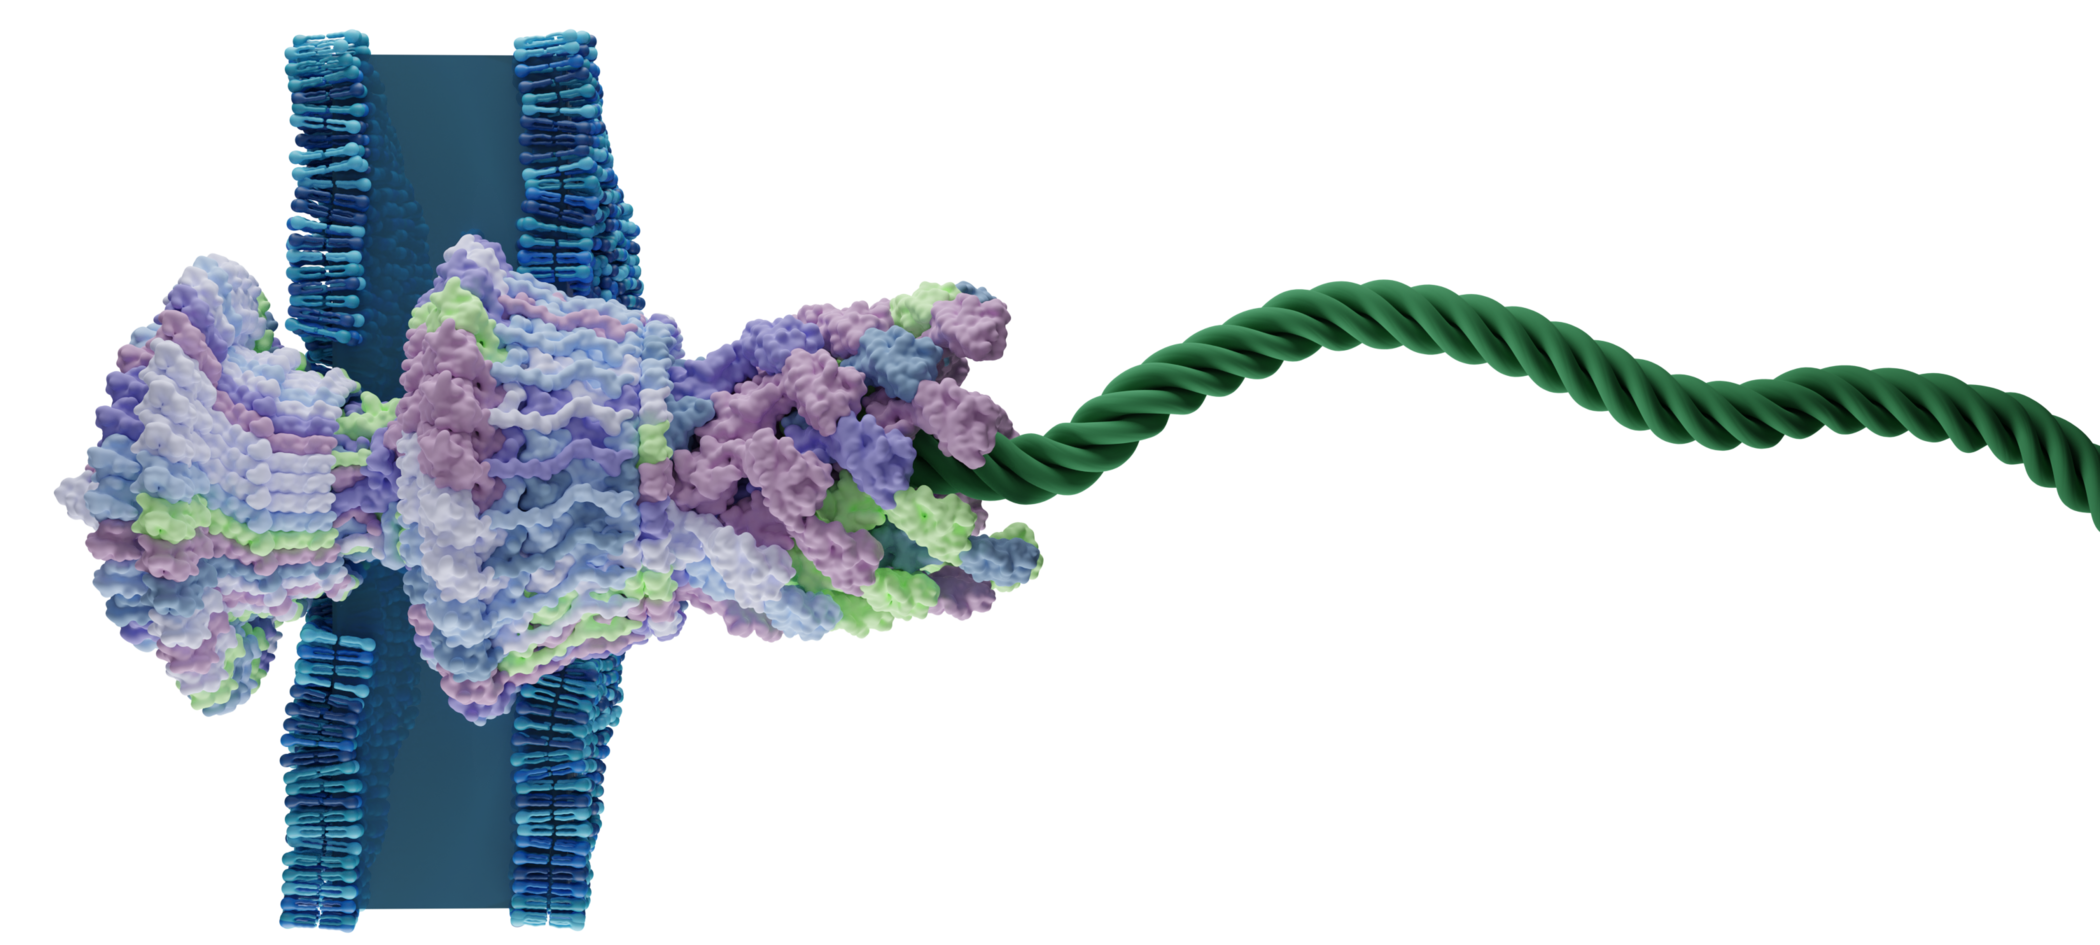
\includegraphics[width=0.30\textwidth]{Figures/flagella.png}
  \end{center}
  \caption{;laskdjfal;s kjdf;a lskdfjl;askjdfl; askdfl;kasjdf w}
\end{wrapfigure}

molecular machines, flagella of bacterio (image of goodsel), synthetic is difficult.
dissipating heat, soft large structures.  polymers, DNA.

creating a molecular machine DNA and nano pores, aim of the molecular machine is to
perform selective transport of dna through the membrane. This has been done before
following an external bias, but special is that the machine opperates also opposing a
external bias. The physics that makes this special property possible is entropy and will
be discussed futher in detail in later chapters of this thesis.

thesis outline, first chapter is a short introduction to important concepts. chapter two
is a discussion of the dna nanopiston, largely based on the paper recently published by
bayoumi et al. Next adaptation of the model is discussed in chapter 3. The results of
these simulations are discussed in the last chapter.
